\documentclass[11pt, a4paper]{article}

\usepackage[utf8]{inputenc}
\usepackage{amsmath, amssymb}
\usepackage{algorithm}
\usepackage{algpseudocode}
\DeclareMathOperator{\diag}{diag} 
\usepackage{graphicx}
\usepackage{hyperref} 

\title{A connectivity modelling toolset for ecological and geospatial edge computing}
\author{Alex Southgate}
\date{\today}

\begin{document}

\maketitle

\begin{abstract}
Circuit theory has been successfully applied to ecological connectivity modelling, notably via the Circuitscape software, which is typically run locally on a laptop or via a server. For downstream geospatial web applications relying on connectivity analysis, backend infrastructure is required, which can be costly and require advanced data governance. Recent developments in WebAssembly now allow fast C++ or Rust code to be run directly in a sandboxed browser environment for edge computing. We present a WebAssembly/Rust toolset with a geospatial data pipeline and efficient edge-computing implementation of connectivity analysis. This approach may be useful for geospatial modelling software where rasters and memory footprint are small enough for the browser context. Our results show that as expected, Circuitscape solves 1000x1000 raster networks 1-2x faster, but requires further file writes. Accounting for total program runtime, our web implementation can be faster for the given context.
\end{abstract}

\section{Introduction}

The theory of linear circuits has found useful application in ecological connectivity modelling, 
population genetics, and conservation \cite{mcrae2008using, mcrae2006isolation, mcrae2007circuit}, 
especially through the Circuitscape \cite{mcrae2016circuitscape} software. 
Circuit theory offers advantages beyond methods such as least-cost paths (see \cite{mcrae2007circuit}).
At the same time, these modelling approaches can require large compute resources, cloud instances or servers,
and technical expertise for maintenance.

In modern web applications, 
a front-end browser application is often paired with a backend server which performs more computationally expensive jobs. 
When scientific code is deployed into production web applications for practical use by customers (e.g. analysts) 
outside of academia, a backend is required. However, for many applications, maintaining this infrastructure is costly. 
Edge computing means making use of compute close to the `edge' of the cloud, 
which is either close to the user's computer, or the user's computer itself. 
An additional advantage to this paradigm is simplified data governance, as storage of personal data can be avoided if
computation occurs directly in the user's browser.
The problem with performing complex calculations in the browser is that browser code 
(i.e. JavaScript) execution is strictly controlled for security purposes, which has poor performance and filesystem interaction.
To resolve this problem, WebAssembly was recently introduced,
allowing fast C++ or Rust code to be run in a sandboxed browser environment. 
It has previously been argued that WebAssembly is poised to transform scientific computing \cite{perkel2024no}.
In addition, web applications may integrate complex user controls
(e.g. modelling controls directly on a map) that are time consuming to complete using scientific scripts,
requiring expertise not always available to users outside of academia.

WebAssembly has found use in several scientific projects, including: Pyodide, a CPython port, supporting installs of NumPy and SciPy, amongst other packages\cite{pyodide2026};
WebR \cite{webr2026}, a WebAssembly compilation of the R language; ITK-Wasm, for spatial/image analysis \cite{itkwasm2026}. 
Application domains include software for mapping pipeline corrosion \cite{guarneri2024web}, viral genomics \cite{ji2024viralwasm}, or cancer genome visualisation \cite{finney2018chromatic}.


This paper introduces a Rust library and WebAssembly bindings to allow connectivity analysis directly within web applications,
such as geospatial analysis software. We demonstrate reasonable
 performance provided input images fit within browser sandbox memory limits,
 which has potential use for deployed scientific applications.

\section{Methodology}

\subsection{Example datasets and resistance map calculation}

In order to demonstrate the functionality of our WASM toolset, a test region corresponding to a 1~$\text{km}^2$ region centered at
286600E, 79050N (EPSG:27700) was selected. The region includes buildings, roads, and a river. Vector data was obtained from
the UK Ordnance Survey open data \cite{os_data}. 
DSM and DTM LIDAR data was obtained from the UK Environment Agency \cite{ea_lidar_composite_2022}.

For the test resistance map, we use constant resistance parameters for rasterised vector features: 50 for roads (3 pixel buffer), 500 for buildings, 
and 0.5 for rivers (4 pixel buffer).
For raster landscape feature resistance, we took the feature height as resistance. 
These parameters were arbitrary and chosen to introduce variation into the test resistance map inputted into current calculation.
In practice, these parameters can be set freely.

In order to keep the WASM toolset lightweight, we avoid heavy geospatial dependencies. For vector rasterisation, we use
the \texttt{geojson} and \texttt{geo} crates, which are lightweight and have no external dependencies. Handling vector inputs allows
applications with vector data to use the WASM toolset directly, and interface cleanly with vector tile
data such as MVT derived from mbtiles.

\subsection{Benchmarking}

Benchmarking was undertaken on a laptop with an AMD Ryzen 7 5700U, 16G of RAM, Linux 6.8.0-51-generic, and using Google Chrome 150.0.7871.46.
Benchmarking code was wrapped in a React applet which can be run locally and accessed via the code repository. Two benchmarks were run. 
In the first case, a resistance map was generated at 1000$\times$1000 resolution, then downsampled to lower resolutions, and the analysis code run with 5 repeats each.
It was expected that, in the browser context, the first run (`cold start') would be slowest due to V8/WASM JIT compilation engine warm-up (`warm start').

For comparison with Circuitscape, a configuration file was created with \texttt{scenario=advanced}, \texttt{write\_as\_tif=True} and run with 4 threads.
Although this allows Circuitscape to multithread, which our implementation does not exploit, it is conventional to run with multiple threads. 

\subsection{Connectivity model}

We use the methodology introduced by \cite{mcrae2006isolation} to describe connectivity with circuit theory, and a brief summary follows. First, Ohm's law \cite[Ch. 2]{alexander2007fundamentals} is \eqref{eq:ohm} specifies the relationship between voltage $V$, current $I$, and resistance $R$ as $V=IR$. Or, using conductance $C = 1/R$:

\begin{equation}
\label{eq:ohm}
I = CV
\end{equation}

Secondly, for a given node (pixel), the conservation equation (Kirchhoff's equation, see \cite[Ch. 2]{alexander2007fundamentals}) \eqref{eq:conservation} just means that movement in is equal to movement out. This does treat the modelled species as a conserved quantity and the simplest approach ignores e.g. death. Taking $S_i$ as a source at node $i$:

\begin{equation}
\label{eq:conservation}
I_i = \sum_{j \in N(i)} C_{ij}V_{ij} - S_i = 0
\end{equation}

Given these two equations, only voltage differences $V_{ij}$ are unknown. Voltage, as a potential can be assumed to be a scalar quantity for a single node up to some constant, which leads to a system of equations \eqref{eq:system}:

\begin{equation}
\sum_{j \in N(i)} C_{ij}(V_i - V_j) = S_i
\end{equation}

\begin{equation}
\Big(\sum_{j \in N(i)} C_{ij}\Big)V_i - \sum_{j \in N(i)} C_{ij}V_j = S_i
\end{equation}

\begin{equation}
\label{eq:system}
\rightarrow \Big(\mathbf{D_C}- \mathbf{M}\Big)\mathbf{v} = \mathbf{L}\mathbf{v} = \mathbf{s}
\end{equation}

Which is a discrete Poisson problem \cite[Ch. 4]{leveque2007finite}. The matrix $\mathbf{L}$ is the Laplacian. The diagonal elements of $\mathbf{L}$ are precomputed. For ground (sink) nodes, either the corresponding rows can be ignored in calculation and set to zero, or the diagonal elements set to $1$ and off-diagonal to zero. $\mathbf{L}$ is sparse, since only neighboring nodes are connected in the simplest case.

\subsection{Modes}

The simplest run mode is for a source and sink pair, equivalent to a conditional random walk (paths of those that travel from source to sink). If a raster image of source nodes is provided, then the resulting output is connectivity given inputs from the combined input sources, solved together, as in a conventional physical system like electrical circuits. Instead of the combined mode, where current will flow according to the global pressure gradient, some users may choose to intentionally superimpose $n \choose 2$ pairwise simulations from pairs of $n$ nodes, or $n \times m$ simulations between $n$ sources and $m$ sinks. Each approach has different assumptions and interpretation. Each mode has the same underlying mathematical system and solver; in the case of a single pair, only two rows of the matrix $L$ are source/sink; in the case of a raster of currents, many rows are set to sources. Superposition of the different cases can be undertaken in a loop over the chosen sets of pairs.

\subsection{Solver}

Given an $N\times M$ image, the matrix $L$ takes $O(NM)$ space. In Circuitscape, conjugate gradient with algebraic multigrid (CG+AMG) or a Cholesky solver is used via optimised CHOLMOD libraries that are not available in a WASM context. In order to keep the WASM binary small, we implement a conjugate gradient (CG) solver and compare several preconditioners (see below).

A good description of the CG method can be found in \cite{shewchuk1994introduction} or \cite[Ch. 4]{leveque2007finite}. Since we implement it manually for WASM, a brief explanation follows. Solving the system:

\[
\mathbf{L}\mathbf{v} = \mathbf{s}
\]

is equivalent to solving the energy function:

\[
f(\mathbf{v}) = \frac{1}{2} \mathbf{v}^T \mathbf{L}\mathbf{v} - \mathbf{v}^T\mathbf{s}
\]

Since when taking the negative gradient and setting to zero, we get the residual error for our system:

\[
-\nabla f(\mathbf{v}) = \mathbf{s} - \mathbf{L}\mathbf{v} = \mathbf{r}
\]

Stepping in the direction $r$ at step $k$ gives us a new guess.

\[
\mathbf{v}_{k+1} = \mathbf{v}_{k} + \mathbf{\alpha} \mathbf{r}_k
\]

Taking the gradient and choosing an optimal step size $\alpha$ gets to the bottom of the hill for that slice. The next step will be orthogonal to the previous one, since if it were not, the previous one would not have been the furthest (best) possible step. In steepest descent, to get the best step, applying calculus to the energy function it can be shown (see \cite[Ch. 4]{leveque2007finite}) that:

\[
\mathbf{\alpha}_{k} = \frac{\mathbf{r}_{k}^T \mathbf{r}_k}{\mathbf{r}_k^T \mathbf{L}\mathbf{r}_k}
\]

However, stepping maximally in a sequence of orthogonal steps can be inefficient and lead to zig-zag steps. Instead, a kind of moving average or momentum can be applied to the steps. 

\[
\mathbf{p}_{k+1} = \mathbf{r}_{k+1} + \mathbf{\beta}_{k+1}\mathbf{p}_k
\]

In the case of CG, $\beta$ is:

\[
\beta_{k+1} = \frac{\mathbf{r}^T_{k+1}\mathbf{r}_{k+1}}{\mathbf{r}_{k}^T\mathbf{r}_{k}}
\]


\subsubsection{Preconditioning} 

As described in \cite[Ch. 4.3.4]{leveque2007finite}, convergence rate depends on condition number. We solve a transformed system:

\[
\mathbf{M}^{-1}\mathbf{L}\mathbf{v} = \mathbf{M}^{-1}\mathbf{s}
\] 

Where $\mathbf{M}^{-1}$ approximates $\mathbf{L}$, reducing the condition number. 
We compare several preconditioners: a simple diagonal preconditioner with $\mathbf{M} = \diag{\mathbf{L}}$, also known as a Jacobi preconditioner, 
which can be useful for some data \cite{wathen2015preconditioning}; a geometric multigrid (GMG) preconditioner, which is more complex but converges faster \cite{tatebe1993multigrid};
an Alcouffe preconditioner \cite{alcouffe1981multi}, which is better for sharply contrasting features.
We implement these methods directly to reduce WASM dependencies and binary footprint. 

The GMG preconditioner is more complex than the Jacobi preconditioner, which smoothes high-frequency features. It requires computing a correction $\mathbf{e}$ using a sequence of coarse-grained matrices and passing them up. At the lowest resolution, the system is solved using Cholesky decomposition. The algorithm proceeds as follows.
The finest grid is smoothed with a few iterations of a Jacobi smoother. The residual is calculated:

\[
r = \mathbf{s} - \mathbf{L}\mathbf{v}
\]

This residual is passed down to a coarser grid using a restriction operator $R$. 
This will be balanced with a prolongation operator, which is a scaled transpose $P = cR^T$, on the way back up.
These operators are comparable to downsampling and upsampling.
This is applied repeatedly until the coarsest resolution is reached.
Then, the system is solved directly to get the coarse error:

\[
\mathbf{e}_{coarse} = \Big(\mathbf{L}_{coarse}\Big)^{-1}\mathbf{r}_{coarse}
\]

After the coarse error is calculated, it is passed upwards via the prolongation $P$,
which was implemented with bilinear interpolation. The errors are passed up:

\[
\mathbf{e}_{fine} = P\mathbf{e}_{coarse}
\]

\[
\mathbf{v}_{fine} \leftarrow \mathbf{v}_{fine} + \mathbf{e}_{fine}
\]

At the end of each step, post-smoothing is required to balance pre-smoothing. This cycle is referred to as the `V-cycle'. 
Algorithm \ref{alg:gmg_vcycle} shows one cycle.

\begin{figure}[h]
\centering
\hrule
\vspace{0.5em}
\noindent\textbf{Algorithm: Geometric Multigrid V-Cycle Preconditioner Step}
\vspace{0.5em}
\hrule
\vspace{0.5em}
\begin{tabbing}
\quad \= \quad \= \quad \= \quad \= \kill
\textbf{Function} $\text{V}(\mathbf{L}_l, \mathbf{s}_l, \mathbf{v}_l, l)$ \\
\> \> \textbf{if} $l == 0$ \textbf{then}\\
\> \> \> \> \textbf{return} $\mathbf{e}_0 = \text{Solve}(\mathbf{L}_0, \mathbf{s}_0)$ \\
\> \> \textbf{end if} \\
\\
\> \> $\mathbf{v}_l \leftarrow \text{Smooth}(\mathbf{L}_l, \mathbf{v}_l, \mathbf{s}_l)$ \\
\\
\> \> $\mathbf{r}_l = \mathbf{s}_l - \mathbf{L}_l \mathbf{v}_l$ \\
\> \> $\mathbf{s}_{l-1} = R \mathbf{r}_l$ \\
\> \> $\mathbf{v}_{l-1} = \mathbf{0}$ \\
\\
\> \> $\mathbf{e}_{l-1} \leftarrow \text{V}(\mathbf{L}_{l-1}, \mathbf{s}_{l-1}, \mathbf{v}_{l-1}, l-1)$ \\
\\
\> \> $\mathbf{e}_l = P \mathbf{e}_{l-1}$ \\
\> \> $\mathbf{v}_l \leftarrow \mathbf{v}_l + \mathbf{e}_l$ \\
\\
\> \> $\mathbf{v}_l \leftarrow \text{Smooth}(\mathbf{L}_l, \mathbf{v}_l, \mathbf{s}_l)$ \\
\\
\> \> \textbf{return} $\mathbf{v}_l$ \\
\textbf{End Function}
\end{tabbing}
\hrule
\caption{One step of the preconditioner V-cycle}
\label{alg:gmg_vcycle}
\end{figure}


\subsection{Code}

Code can be obtained at \url{https://github.com/asouthgate/wasm-connectivity}. This code contains several simple examples. All results can be easily reproduced by running the React development server, clicking to the benchmark panel, running the benchmarks, and downloading the results.

\section{Results}

Figure \ref{fig:wasm-connectivity} gives an example of a 1000x1000 resistance input and current map output
rendered in a React frontend using raster source mode (`advanced mode') for the test region.
Figure \ref{fig:benchmarking} shows time and memory benchmarks as a function of raster size. As shown,
the CG MG preconditioners were much faster than Jacobi preconditioning, while taking modestly more memory.

\begin{figure}[htb!]
\centering
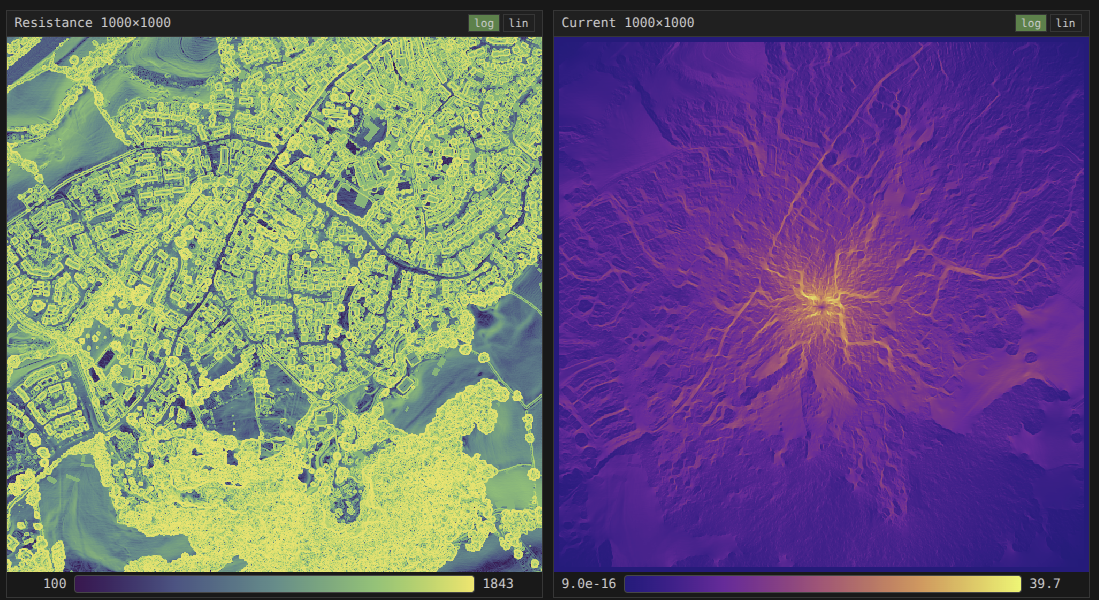
\includegraphics[width=0.8\textwidth]{figures/resistance_current_react.png}
\caption{Example dataset 1000x1000 log resistance and log current maps rendered using a React frontend with WASM connectivity library, computed in 6.52 seconds.}
\label{fig:wasm-connectivity}
\end{figure}


\begin{figure}[htb!]
\centering
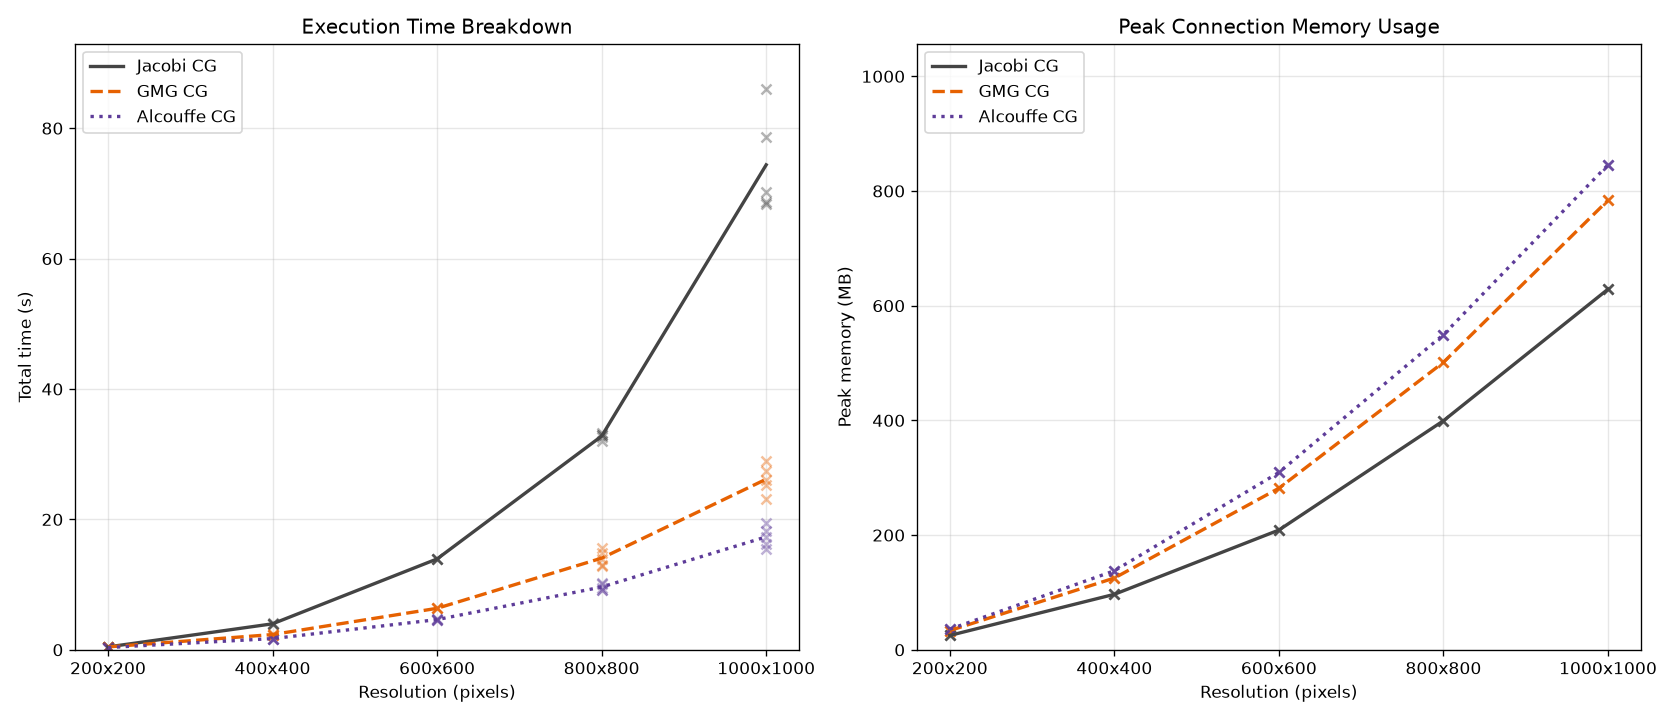
\includegraphics[width=0.8\textwidth]{figures/benchmarking.png}
\caption{Time and memory comparison across resolutions for each solver. Both MG solvers converge much more quickly, while only taking marginally more memory. Individual data points are shown as crosses, the mean as solid lines.}
\label{fig:benchmarking}
\end{figure}

Figure \ref{fig:comparison} shows a side-by-side comparison of a Circuitscape current map produced from
the same resistance map input with a zero-volt ground, showing comparable results.

\begin{figure}[htb!]
\centering
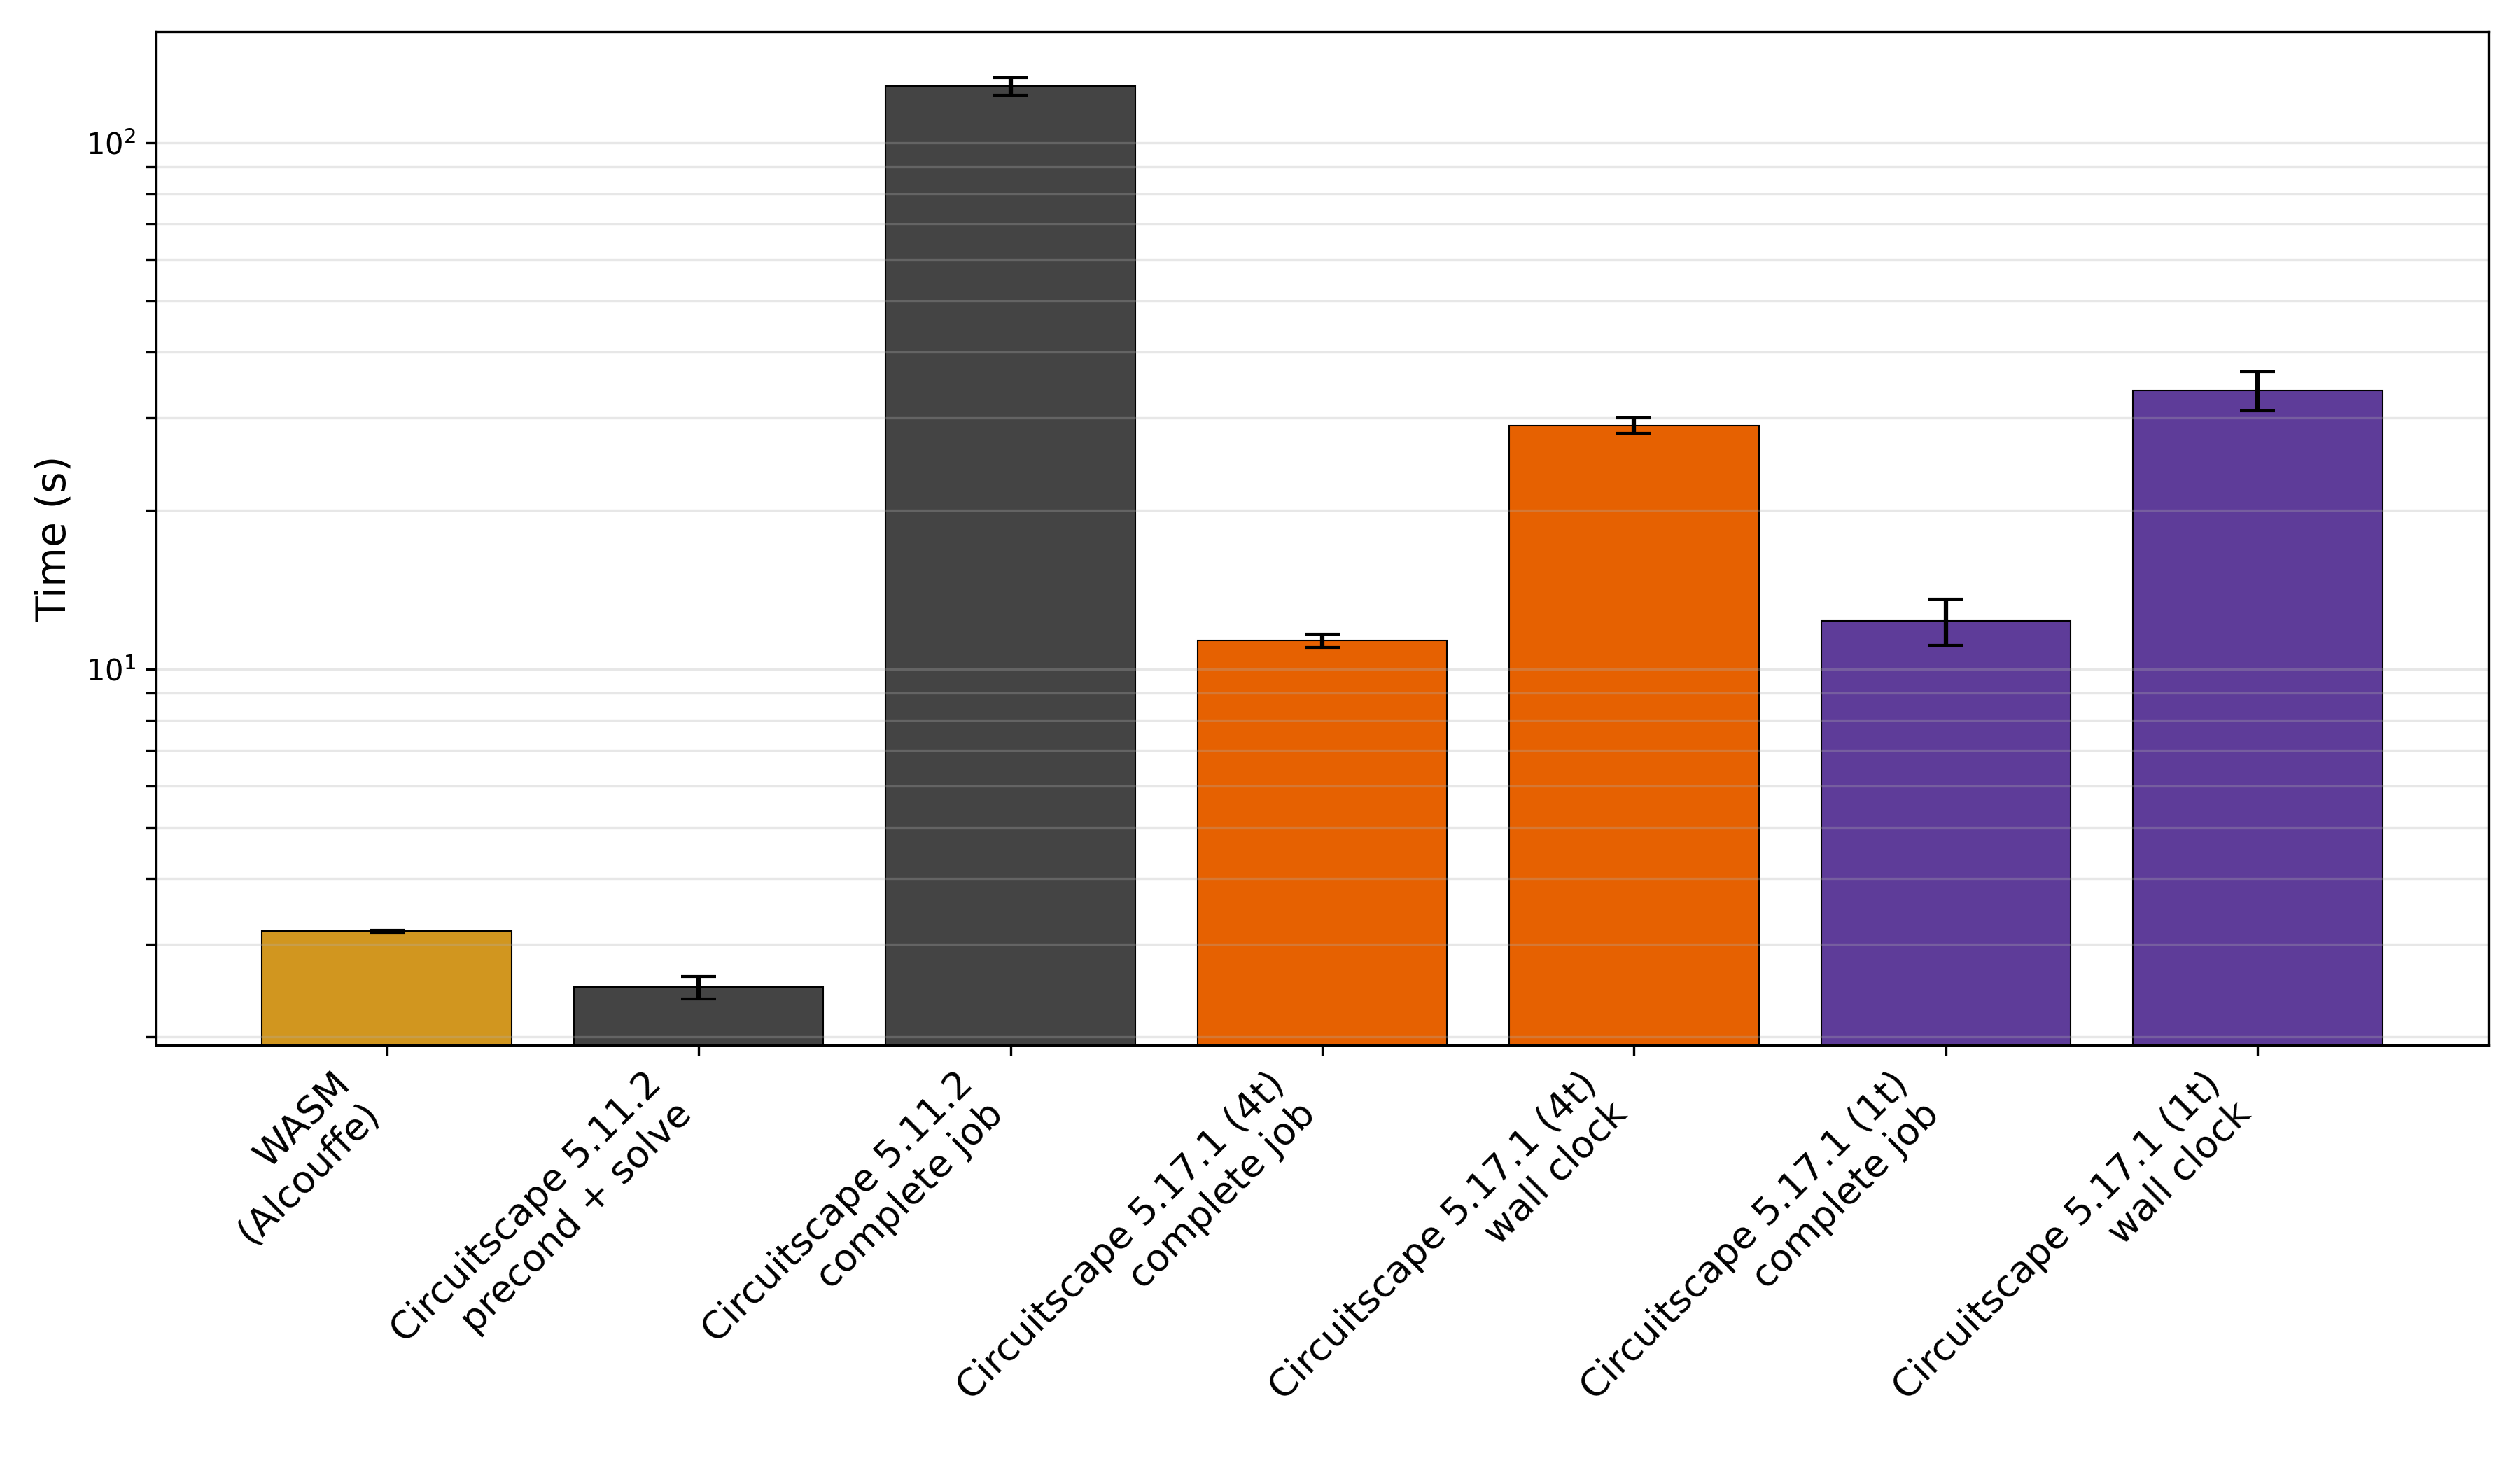
\includegraphics[width=0.8\textwidth]{figures/cs_vs_wasm.png}
\label{fig:cs_runtime}
\caption{Runtime comparison between Circuitscape and our WASM implementation for a 500x500 test raster. Circuitscape took 2.48 seconds ($\pm$0.12), versus 3.79 ($\pm$0.38) for WASM (Alcouffe). Overall program runtime for Circuitscape exceeded both. Error bars give standard deviation. }
\end{figure}

As demonstrated by Figure \ref{fig:cs_runtime}, Circuitscape solvers are much quicker than the presented
WASM browser solvers. The average time for WASM (Alcouffe) was 3.79 seconds, compared to 2.48 seconds for the 
preconditioner building and solve step in Circuitscape.
However, the total runtime of Circuitscape including post-solving steps was much slower, at 128.11s.
In the web browser context which we utilise, we do not have to write the data to file, and presentation in 
the browser is near-instantaneous.
As such, provided there is sufficient memory, these results show our implementation can out-perform
circuitscape in a web-application context, even though the circuitscape solver is faster,
especially if the solver does not dominate the time taken for an
analysis round trip from browser to server and back.

\begin{figure}[htb!]
\centering
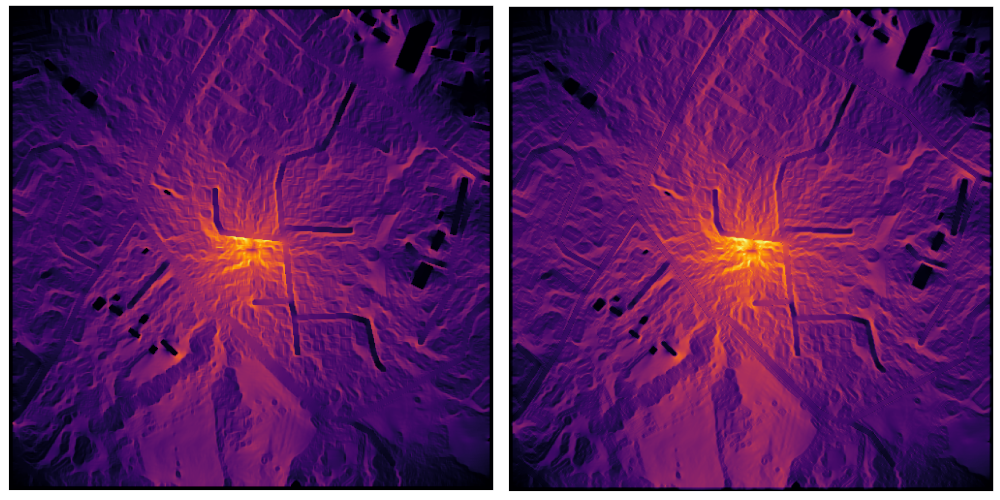
\includegraphics[width=0.8\textwidth]{figures/comparison_cs_alc.png}
\caption{Side-by-side comparison showing log current maps produced by Circuitscape (left) and our implementation (right), to show consistency.}
\label{fig:comparison}
\end{figure}



\section{Discussion}

We present a WASM/Rust connectivity library for interactive geospatial edge-computing by implementing the core Circuitscape connectivity model with
a custom conjugate gradient solver with geometric multigrid preconditioning. This method can be integrated into geospatial web applications,
allowing fast connectivity modelling in the resource-limited browser WASM context.

Although Circuitscape solves the linear equations for this problem quicker than our implementation, the post-solve steps and total runtime exceeded
that of our WASM implementation for the datasets examined. As such, our implementation is advantageous in a web context, 
and removes the need for a backend server and data governance.
Different solvers have different performance on different input matrices. While this implementation gives reasonable performance for the
tested data, it is likely to vary with different rasters depending on the type of features they contain.

Limitations of the WASM environment are primarily constraints in memory, CPU, and binary size. Traditionally, scientific software relies on 
highly optimised libraries such as BLAS or, in the case of Circuitscape, CHOLMOD or AMG libraries. In principle, this is possible for WASM, but it is not straightforward.
Projects like Pyodide \cite{pyodide2026} demonstrate the work required for compiling existing packages into WASM executables. 
In addition, for front-end web applications, it is often important that data transfer is minimised to enable responsive pages.

Some of the methods applicable in this paper, as image processing codes, could be suitable for GPU acceleration, such as through WebGPU. Dedicated GPU
cards offer acceleration for highly parallel workloads. While dedicated GPU cards can be expensive and in short supply, consumer hardware often includes
integrated GPU that can be exploited for acceleration provided a suitable workload. In addition, it is possible to implement multithreaded applications
using shared buffers and web workers, which could also be explored in future work.
Future work could also explore alternative solver methods and optimisations for the browser context, such as via using mixed-precision or SIMD instructions.

\section{LLM disclaimer}

This paper was written by hand without LLM generation. Code and research was developed with LLM assistance.

\bibliographystyle{plain} 
\bibliography{refs} 

\end{document}
